\chapter{Synchronization mechanisms analysis\label{chap:sync_mechanisms}}

As we stated in the previous chapter, the main goal of this thesis is to 
design and develop new migration mechanisms that scale well while the number
of underlying cores increases. So, we can't leave aside a detailed description
of the various synchronization mechanisms used to ensure a correct interaction
between multiple threads of execution. In particular, we are going to detail
the facilities that the Linux kernel provides to developers.

After that, we will explain a novel (and widely applicable) framework to 
efficiently manage  concurrent accesses to a shared data structures, 
called \emph{flat combining}.

\section{Kernel locking techniques\label{sec:kernel_lock}}

The fundamental issue surrounding locking is the need to provide mutual exclusion 
in certain code paths in the kernel. These code paths, called \emph{critical sections},
require some combination of concurrency or re-entrancy protection and proper ordering
with respect to other events. The typical result without proper locking is called a
\emph{race condition}: the output is dependent on the sequence of events.
To avoid race conditions we need to rely on locking. The Linux kernel provides a 
family of locking primitives that developers can use to write safe and efficient code.

\subsection{SMP and UP Kernel\label{sec:SMP_UP}}
Depending on the configuration used to compile the kernel, Linux can be configured to
be used in a uniprocessor (\emph{UP}) or in a multiprocessor (\emph{SMP}) environment.
Some locking issues arises only in a \emph{SMP} kernel, where we have real parallelism,
that is, more than one instructions are executed at the exact same time. But even in a
\emph{UP} kernel we may have some locking issues: if it is compiled with preemption enabled,
a kernel can preempt itself, thus leading to the need of locking usage.

Linux locking primitives are written in order to ensure proper synchronization with all
kinds of kernel, thanks to the conditional compilation enabled by two macros:

\begin{itemize}
\item \texttt{CONFIG\_SMP} to enable kernel \emph{SMP} support
\item \texttt{CONFIG\_PREEMPT} to enable kernel preemption support
\end{itemize}

In the following analysis we will refer to a kernel with both two macros defined.

\subsection{Atomic operators\label{sec:atomic_ops}}
Atomic operators are maybe the simplest of the approaches to kernel synchronization
and thus probably the easiest to understand and use. In addition to this, they are the
building blocks of the kernel's locks.

Atomic operators are operations, like add and subtract, which execute in one uninterruptible
operation. There are two different subsets of atomic operations: methods that operates
on integers and methods that operates on bits. For the sake of simplicity, we are going to 
describe only the first subset.

The most important atomic operations are listed in the following ~Listing\ref{lst:atomic_ops}.

\begin{lstlisting}[language=C, caption={Atomic operations on integer},
			label={lst:atomic_ops}]

void atomic_set(atomic_t *v, int i);
int atomic_read(const atomic_t *v);
void atomic_add(int i, atomic *v);
void atomic_sub(int i, atomic_t *v);
int atomic_cmpxchg(atomic_t *v, int old, int new);

\end{lstlisting}

The above primitives work on a integer variable (encapsulated in \texttt{atomic\_t}
type), that extends on 32 bits on most hardware architectures. Others atomic 
operations for 64-bit variables are also available.

The semantics of the above operations is quite straightforward, but there is one of
those that deserves a futher explanation. The \texttt{atomic\_cmpxchg} operation is
fundamental, because it allows to realize the so called \emph{CAS} (Compare-And-Swap)
operation: the value of the memory location addressed by \texttt{v} pointer is atomically
exchanged with the \texttt{new} value iff memory contains the \texttt{old} value. 
If the exchange actually takes place, \texttt{atomic\_cmpxchg} returns \texttt{old}
value, otherwise it returns a different value. This operation is also particular because
it is the only one among the above that issues a full memory barrier. We will discuss
about memory barriers in Section~\ref{sec:mem_barriers}.

\subsection{Spinlocks\label{sec:spinlocks}}

For anything more complicated than the basic arithmetic operations, a more complete
locking solutions is needed. The most common locking primitive in the kernel is the 
spinlock. The spinlock is a very simple single-holder lock. If a process attempts 
to acquire a spinlock and it is unavailable, the process will keep trying (that is:
spinning) until it can acquire the lock. This simplicity leads to a small and fast
lock.

An example of usage is in Listing~\ref{lst:spinlock_ops}.

\begin{lstlisting}[language=C, caption={Spinlock operations},
			label={lst:spinlock_ops}]

spinlock_t lock = SPIN_LOCK_UNLOCKED;
unsigned long flags;

spin_lock_irqsave(&lock, flags);
/* critical section */
spin_unlock_irqrestore(&lock, flags);

\end{lstlisting}

The use of \texttt{spin\_lock\_irqsave} will disable interrupts locally and implement the
spinlock on \emph{SMP} systems. With a call to \emph{spin\_unlock\_irqrestore}, interrupts
are restored to the state when the lock was acquired. All of the above spinlocks assume
the data they are protecting is accessed in both interrupt handlers and normal kernel
code. If that critical section is accessed only in user-context kernel code (like a 
system call) the variants \texttt{spin\_lock()} and \texttt{spin\_unlock} have to be 
used instead of the above.

In Linux, spinlocks are not recursive, as in other operating systems: the
programmer has to carefully deal with them in order to avoid potential deadlocks.

Spinlocks should be used to lock data in situations where the lock is not held for
a long time: a waiting process will spin, doing nothing, waiting for the lock to be
available.

Another fundamental API provided by Linux is \texttt{spin\_trylock\_irqsave}: it is a 
non-blocking variant of \texttt{spin\_lock\_irqsave} that returns zero if the lock is
successfully acquired, otherwise it returns a non-zero value without spin. In the
subsequent chapters, we will see how this primitive can effectively used to implement
lock-free solutions for shared data structures concurrency management.

\subsection{Semaphores\label{sec:semaphores}}

Semaphores in Linux are implemented as sleeping locks: a task that fails to acquire the
semaphore due to contention is forced to sleep. Because of this, semaphores are usually
used in situations where the lock-held time may be long. Conversely, since they have a
non negligible overhead of putting a task to sleep and subsequently waking it up, they
should not be used where the lock-hold time is short. On the other hand, a task can 
safely block while holding a semaphore, so they can be used to synchronize user contexts.

In Linux, semaphores are represented by a structure, \texttt{struct semaphore}, that
contains:

\begin{itemize}

\item a pointer to a \emph{wait queue}
\item a \emph{usage count}

\end{itemize}

The wait queue is a list of processes blocking on the semaphore, while the usage count 
is the number of concurrently allowed holders. If it is negative, the semaphore is
unavailable and the absolute value of the usage count is the number of processes
blocked on the wait usage.

The primitives used to manage a semaphore is showed in Listing~\ref{lst:semaphore_ops}.

\begin{lstlisting}[language=C, caption={Semaphore operations},
			label={lst:semaphore_ops}]

void sema_init(struct semaphore *sem, int val);
int down_interruptible(struct semaphore *sem);
void down(struct semaphore *sem);
void up(struct semaphore *sem);

\end{lstlisting}

The \emph{sema\_init} simply initializes the semaphore. The \emph{up} function is used to
release the semaphore, incrementing the usage count. If the new value is greater than or
equal to zero, one or more tasks on the wait queue will be woken up.

To attempt to acquire a semaphore, we have to use one among \texttt{down\_interruptible}
and \texttt{down} functions: the former decrements the usage count of the semaphore and,
if the new value is less than zero, the calling process is added to the wait queue and
blocked. If the new value is greater or equal to zero, the process obtains the semaphore
and the call returns 0. If a signal is received while blocking, the call returns the
\texttt{-EINTR} error code and the semaphore is not acquired. The latter performs almost
the same, except that it puts the calling task into an uninterruptible sleep: a signal
received by a process in such a status is ignored.

\subsection{Reader/Writer locks\label{sec:rw_locks}}

In addition to spinlocks and semaphores, Linux provides reader/writer variants that divide
lock usage into two groups: reading and writing. Since it is safe for multiple threads to
read data concurrently, so long as nothing modifies the data, reader/writer locks allow
multiple concurrent readers but only a single writer (with no concurrent readers). If the
data accesses can be clearly divided into reading and writing patterns, especially with 
a greater amount of reading than writing, the reader/writer locks are to be preferred.
In Listings~\ref{lst:rwspinlocks} we provide an usage example of reader/writer spinlocks and
reader/writer sempahores, respectively.

\begin{lstlisting}[language=C, caption={Reader/Writer Spinlocks},
                        label={lst:rwspinlocks}]

rwlock_t rw_lock = RW_LOCK_UNLOCKED;

read_lock(&rw_lock);
/* critical section (read only) */
read_unlock(&rw_lock);

write_lock(&rw_lock);
/* critical section (read and write) */
write_unlock(&rw_lock);

\end{lstlisting}


\begin{lstlisting}[language=C, caption={Reader/Writer Semaphores},
			label={lst:rwsem}]

struct rw_semaphore rw_sem;
init_rwsem(&rw_sem);

down_read(&rw_sem);
/* critical section (read only) */
up_read(&rw_sem);

down_write(&rw_sem);
/* critical section (write only) */
up_write(&rw_sem);

\end{lstlisting}

Use of those kind of locks, where appropriate, is an appreciable optimization.

\section{Memory barriers\label{sec:mem_barriers}}

Before discussing memory barriers, we need to introduce the mechanisms that rules
the interaction between CPUs and memory in a multiprocessor environment.
After that, it will be clear how important memory barriers are while developing lock-free
solutions in a multicore environment.

For further details about memory barriers see~\cite{Mckenney2009}.

\subsection{Abstract memory access model\label{sec:mem_barr_model}}

Consider the abstract model of the system in \figurename~\vref{fig:abstract_system_model}.

\begin{figure}[htbp]
    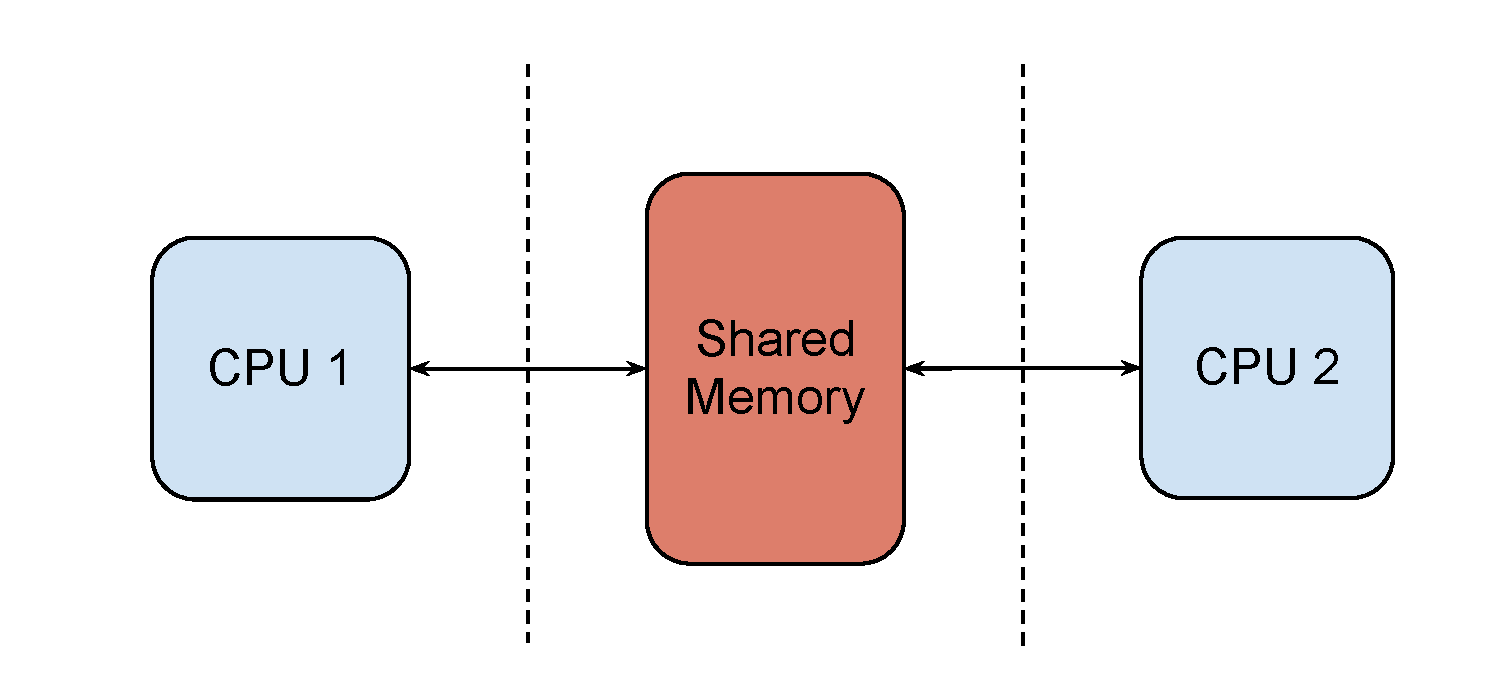
\includegraphics[width=\columnwidth]{images/abstract_system_model} 
    \caption{An abstract model of a multiprocessor system.}
    \label{fig:abstract_system_model}
\end{figure}

Each CPU executes a program that generates memory access operations. In the abstract CPU,
memory operation ordering is very relaxed: a CPU may actually perform the memory operations
in an order it likes, provided \emph{program causality} appears to be mantained. Similarly,
the compiler may also arrange the instructions it emits in any order it like, provided
it does not affect the apparent operation of the program.

So, in the above diagram, the effects of the memory operations performed by a CPU are
perceived by the rest of the system as the operations cross the interface between the CPU
and rest of the system.\\
As an example, consider the sequence of events shown in Table~\ref{tab:cpu_ops}.

\begin{table*}[htb]
\centering
\small
\renewcommand{\arraystretch}{1.5}
\begin{tabular}{|c|c|}
        \hline \textbf{CPU 1}& \textbf{CPU 2}\\[5pt]
	\hline \multicolumn{2}{|c|}{ \{A == 1; B == 2\} }\\ 
        \hline A = 3; & x = A;\\
        \hline B = 4; & y = B;\\
        \hline
\end{tabular}

\caption{A sequence of memory operations performed by two CPUs}
\label{tab:cpu_ops}
\end{table*}

The set of accesses as seen by the memory system can be arranged in 24 different combinations,
some of them are showed below as examples.

\begin{center}
STORE A=3, STORE B=4, x=LOAD A$\rightarrow$3, y=LOAD B$\rightarrow$4;\\
STORE A=3, STORE B=4, y=LOAD B$\rightarrow$4, x=LOAD A$\rightarrow$3;\\
STORE A=3, x=LOAD A$\rightarrow$3, STORE B=4, y=LOAD B$\rightarrow$4;\\
STORE A=3, x=LOAD A$\rightarrow$3, y=LOAD B$\rightarrow$2, STORE B=4;\\
STORE A=3, y=LOAD B$\rightarrow$2, STORE B=4, x=LOAD A$\rightarrow$3;\\
STORE A=3, y=LOAD B$\rightarrow$2, x=LOAD A$\rightarrow$3, STORE B=4;\\
STORE B=4, STORE A=3, x=LOAD A$\rightarrow$3, y=LOAD B$\rightarrow$4;\\
...
\end{center}

Since all of the above permutations are eligible, the final result can be one of the
subsequent four different combinations of values:

\begin{center}
x == 1, y == 2\\
x == 1, y == 4\\
x == 3, y == 2\\
x == 3, y == 4
\end{center}

Furthermore, the stores committed by a CPU to the memory system may not be perceived
by the loads made by another CPU in the same order as the stores were committed.

As a further example, consider the sequence of events showed in Table~\ref{tab:cpu_ops2}

\begin{table*}[htb]
\centering
\small
\renewcommand{\arraystretch}{1.5}
\begin{tabular}{|p{4cm}|p{4cm}|}
        \hline \textbf{CPU 1}& \textbf{CPU 2}\\[5pt]
	\hline \multicolumn{2}{|c|}{ \{A == 1, B == 2, C == 3, P == \&A, Q == \&C\} }\\	
        \hline B = 4; & Q = P;\\
        \hline P = \&B; & D = *Q;\\
        \hline
\end{tabular}

\caption{Another sequence of memory operations performed by two CPUs}
\label{tab:cpu_ops2}
\end{table*}

There is an obvious data dependency here, as the value loaded into D depends on the
address retrieved from P by CPU 2. At the end of the sequence, any of the following
results are possible:

\begin{center}
(Q == \&A) and (D == 1)\\
(Q == \&B) and (D == 2)\\
(Q == \&B) and (D == 4)
\end{center}

Note that CPU 2 will never try and load C into D because the CPU will load P into Q
before issuing the load of *Q.

\subsection{CPU guarantees\label{sec:mem_barr_CPU_guar}}

Since we have stated that any CPU may reorder instructions until it doesn't affect
\emph{program causality}, let's now list the minimal guarantees that a programmer
may be expected from a CPU:

\begin{itemize}

\item On any given CPU, dependent memory accesses will be issued in order, with
respect to itself. This means that for:

\begin{center}
Q = P; D = *Q;
\end{center}

the CPU will issue the following memory operations:

\begin{center}
Q = LOAD P, D = LOAD *Q
\end{center}

and always in that order.

\item We say that loads and stores operations \emph{overlap} if they are targeted at
overlapping pieces of memory. So, overlapping loads and stores within a particular 
CPU will appear to be ordered within that CPU. This means that for:

\begin{center}
a = *X; *X = b;
\end{center}

the CPU will only issue the following sequence of memory operations:

\begin{center}
a = LOAD *X, STORE *X = b
\end{center}

And for:

\begin{center}
*X = c; d = *X;
\end{center}

the CPU will only issue:

\begin{center}
STORE *X = c, d = LOAD *X
\end{center}

\end{itemize}

Besides those, there are a number of things that \textbf{must} or \textbf{must not}
be assumed:

\begin{itemize}

\item It \textbf{must not} be assumed that \emph{independent} (that is, not overlapping)
loads and stores will be issued in the order given.

\item It \textbf{must} be assumed that overlapping memory accesses may be merged or
discarded. This means that for:

\begin{center}
*A = X; Y = *A;
\end{center}

we may get any one of the following sequences:

\begin{center}
STORE *A = X; Y = LOAD *A;
STORE *A = Y = X;
\end{center}

\end{itemize} 

\subsection{Behaviour and varieties of memory barriers}

As seen above, independent memory operations are effectively performed in random order,
this can be a problem for CPU to CPU interaction (and even for interaction with the
I/O subsystem). What is required is some way to instruct the compiler and
the CPU to restrict the order.

Memory barriers have been created for this purpose: they impose a perceived \emph{partial
ordering} over the memory operations on either side of the barrier.

Such enforcement is important because the CPUs can use a variety of tricks to improve
performance, including reordering, deferral and combination of memory operations,
speculative loads, speculative branch prediction and various type of caching. Memory
barriers are thus used to override or suppress these tricks, allowing the code to sanely
control the interaction of multiple CPUs.

Memory barriers come in four basic varieties:

\begin{description}
\item[Write memory barriers] These barriers gives the guarantee that all STORE operations
specified before the barrier will appear to happen before all the STORE operations
specified after the barrier with respect to the other CPUs of the system.

A write barrier is a partial ordering on stores only: it is not required to have any
effects on load.
\item[Data dependecy barriers] They are a weaker form of read barrier. In the case
where two loads are performed such that the second depends on the result of the first
(e.g.: the first load retrieves the address to which the second load will be directed),
a data dependency barrier would be required to make sure that the target of the second
load is updated before the address obtained by the first load is accessed.

A data dependecy barrier is a partial ordering on interdependent loads only; it is not
required to have any effects on stores, independent loads or overlapping loads.
\item[Read memory barriers] Those barriers are like data dependency type plus a guarantee
that all the LOAD operations specified before the barrier will appear to happen before
all the LOAD operations specified after the barrier with respect to the other CPUs of
the system.

A read barrier is a partial ordering on loads only; it is not required to have any effect
on stores.
\item[General memory barriers] A general memory barrier gives a guarantee that all the
LOAD and STORE operations specified before the barrier will appear to happen before all
the LOAD and STORE operations specified after the barrier with respect to the other CPUs
of the system.

A general memory barrier implies both read and write memory barriers, and so can substitute
for either.
\end{description}

There are also a couple of implicit varieties:

\begin{description}
\item[LOCK operations] This acts as one-way permeable barrier. It guarantees that all
memory operations after the LOCK operation will appear to happen after the LOCK operation
with respect to the other components of the system.
\item[UNLOCK operations] This also acts as a one-way permeable barrier. It guarantees that
all memory operations before the UNLOCK operation will appear to happen before the UNLOCK
operation with respect to the other components of the system.

LOCK and UNLOCK operations are guaranteed to appear with respect to each other strictly
in the order specified.
\end{description}
It is important to note that these are \emph{minimum} guarantees that barriers provide.
Different architectures may give more substantial guarantees, but they may not be
relied upon outside of architecture specific code in Linux.

\subsection{SMP barriers pairing}

It is important to point out that there are certain things that the Linux kernel memory
barriers does not guarantee:

\begin{itemize}
\item There is no guarantee that any of the memory accesses specified before a memory barrier
will be complete by the completion of a memory barrier instruction: the barrier can be
considered to draw a line in that CPU's access queue that accesses of the appropriate type
may not cross.
\item There is no guarantee that issuing a memory barrier on one CPU will have any direct
effect on another CPU or any other hardware in the system. The indirect effect will be the
order in which the second CPU sees the effects of the first CPU's accesses occur.
\item There is no guarantee that a CPU will see the correct order of effects from a second
CPU's accesses, even if the second CPU uses a memory barrier, unless the first CPU also
uses a matching memory barrier.
\end{itemize}

Starting from the last two points, we can understand that, when dealing with CPU to CPU 
interactions, certain types of memory barrier should always be paired.

A write barrier should always be paired with a data dependency barrier or read barrier,
though a general barrier would also be viable. Similarly, a read barrier or a data
dependency barrier should always be paired with at least a write barrier, though,
again, a general barrier is viable.

An example of such pairing is the sequence of events reported in 
Figure~\vref{fig:SMP_barrier_pairing}.

\begin{figure}[htbp]
    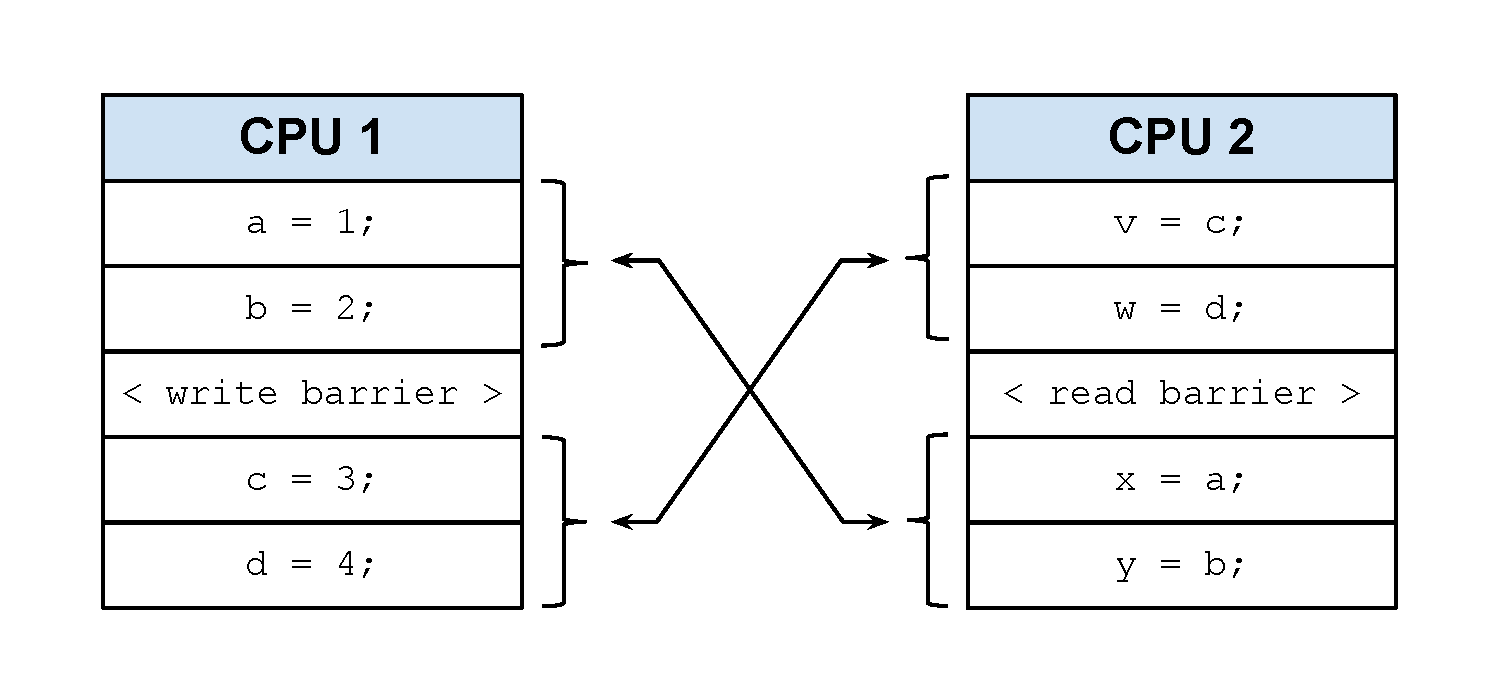
\includegraphics[width=\columnwidth]{images/SMP_barrier_pairing}
    \caption{A sequence of memory operations where SMP barrier pairing is required.}
    \label{fig:SMP_barrier_pairing}
\end{figure}

Note that the stores before the write barrier would normally be expected to ``match'' the
loads after the read barrier or the data dependency barrier, and vice versa.

\subsection{Explicit Linux kernel barriers\label{sec:barrier_Linux}}

The Linux kernel has a variety of different barriers that act at different levels:

\begin{itemize}

\item Compiler barriers: Linux has an explicit compiler barrier function that prevents the
compiler from moving the memory accesses either side of it to the other side:

\begin{center}
\texttt{barrier()}
\end{center}

This is a general barrier.
The compiler barrier has no direct effect on the CPU, which may then reorder things however
it wishes.

\item CPU memory barriers: Linux has eight basic CPU memory barriers, as we can see in
Table~\ref{tab:Linux_mem_barriers}.

\end{itemize}

\begin{table*}[htb]
\centering
\small
\renewcommand{\arraystretch}{1.5}
\begin{tabular}{|p{3cm}|p{5cm}|p{5.5cm}|}
        \hline \textbf{Type}& \textbf{Mandatory}& \textbf{SMP Conditional} \\[5pt]
        \hline General & \texttt{mb()} & \texttt{smp\_mb()} \\
        \hline Write & \texttt{wmb()}  & \texttt{smp\_wmb()}  \\
        \hline Read & \texttt{rmb()} & \texttt{smp\_rmb()} \\
	\hline Data Dependency & \texttt{read\_barrier\_depends()} & \texttt{smp\_read\_barrier\_depends()} \\
	\hline
\end{tabular}

\caption{Linux kernel memory barriers}
\label{tab:Linux_mem_barriers}
\end{table*}

All memory barriers, except the data dependency barriers imply a compiler barrier.

SMP memory barriers are reduced to compiler barriers on uniprocessor compiled systems
because it is assumed that a CPU will appear to be self-consistent, and will order
overlapping accesses correctly with respect to itself. So, SMP memory barriers must
be used to control the ordering of references to shared memory on SMP systems, though
the use of locking instead is sufficient.

Mandatory barriers should not be used to control SMP effects, since mandatory barriers
unnecessarily impose overhead on UP systems.

\subsection{Implicit kernel memory barriers\label{sec:implicit_kernel_barriers}}

Some of the other functions in the Linux kernel imply memory barriers, amongst which
are locking and scheduling functions.

It is importanto to point out that all the atomic operations that modify some state
in memory and return information about the state (old or new) imply an SMP-conditional
general memory barrier (that is: a call to  \texttt{smp\_mb()}) on each side of the
actual operation. Among these operations we find \texttt{atomic\_cmpxchg}, explained in
Section~\ref{sec:atomic_ops}.

\section{Flat combining\label{sec:flat_combining}}

\emph{Flat combining}~\cite{Hendler2010} is a new synchronization paradigm recently introduced by D. Hendler,
I. Incze, N. Shavit and M. Tzafrir, that aims at reducing the synchronization overhead while
accessing a shared data structure with multiple threads of execution.

The idea behind \emph{Flat combining} is to have a given sequential data structure, named
\emph{D}, protected by a lock and have an associated dynamic publication list of a size
proportional to the number of threads that are concurrently accessing it. Each thread accessing
\emph{D} for the first time adds a thread-local publication record to the list, and publishes
all its successive accesses or modifications requests using a write to the request field
of its publication record. In each access, after writing its request, it checks if the shared
lock is free, and if so attempts to acquire it using a \emph{CAS} (Compare-And-Set) operation.
A thread that succesfully acquires the lock becomes a \emph{combiner}: 

\begin{itemize}
\item it scans the list, collecting pending requests;
\item applies the \emph{combined requests} to \emph{D};
\item writes the results back to the threads' request fields in the associated publication records;
\item finally, it releases the lock.
\end{itemize}

Otherwise, a thread that detects that some other thread already owns the lock, spins on its record,
waiting for the owner to return a response in the request field, at which point it knows the
published request has been applied to \emph{D}. Once in a while, a combining thread will
perform a cleanup operation on the publication list. During this cleanup it will remove records
not recently used, so as to shorten the length of the combining traversals. Thus, in each repeated
access request, if a thread has no active publication record, it will use it, and if not, it will
create a new record and insert it into the list.

We can assert that flat combining is a concurrency management framework that can be
adapted to many sequential data structures.

Unfortunately, not all the data structures are suited to be managed with this framework: the authors
say that any data structure such that \emph{k} operations on it, each taking time $\delta$, can be
combined and then applied in time \emph{less than $k \cdot \delta$}, is a valid candidate to benefit
from flat combining. So, as an example, most kind of search trees do not fit the above formula.

Furthermore, even in beneficially combinable structures, the ones that have high levels of mutation on
the data structure will be rapidly beaten in performance by a finely-grained lock implementation.

Finally, we have to consider that such implementation introduces an asynchronous programming 
pattern: a thread that want to issue a sort of \emph{find} operation on the data structure may have 
to wait until a combiner thread return the searched value in his publication record.
